%\documentclass[11pt,a4paper,draft,oneside]{report}
\documentclass[11pt,a4paper]{report}

\usepackage{booktabs}
\usepackage{subfiles}
\usepackage{pdfpages}
\usepackage{setspace}

\doublespacing
%\onehalfspacing
%\singlespacing

\begin{document}
\pagestyle{empty}

\title{Mah Dissertat'n}
\author{Mark Pinese}
\date{\today}

\maketitle

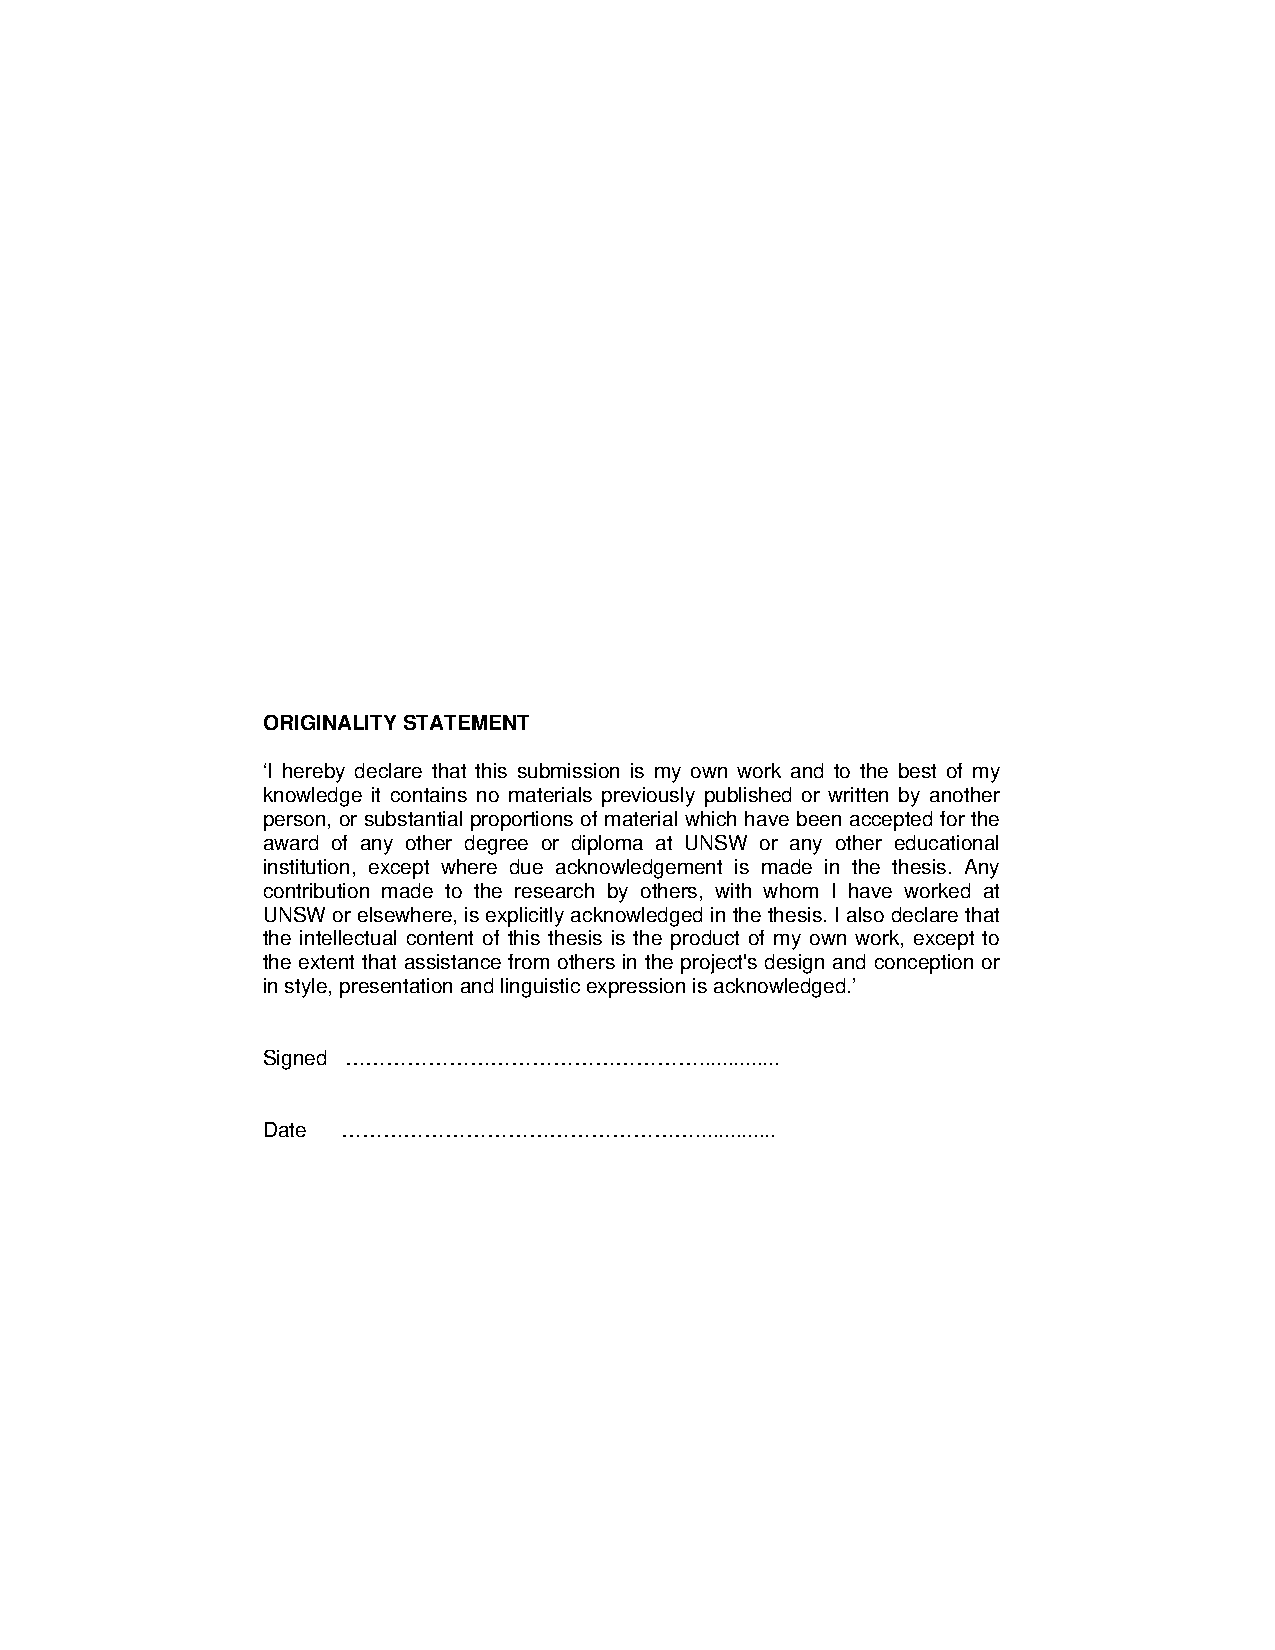
\includepdf[pages={1}]{resources/originalitystatement_1.pdf}

\chapter*{Acknowledgements}
\thispagestyle{empty}
\pagenumbering{gobble}

\begin{abstract}
Da abstract.
\end{abstract}

\pagenumbering{roman}
\setcounter{page}{1}
\tableofcontents
\listoffigures
\listoftables

\chapter*{Abbreviations}

\pagenumbering{arabic}

\begin{tabular}[c]{ l | l }
  CPV           & Clinico-pathological variable \\
  CNV           & Copy number variation \\
  LOH           & Loss of heterozygosity \\
  SNV           & Single nucleotide variant \\
  Indel         & Insertion / deletion \\
  LA-BQSR       & Local alignment and base quality score recalibration \\
  BAM (file)    & Binary sequence alignment / map format \\
\end{tabular}


\chapter*{Software versions}
Unless otherwise specified, the following versions of software were used in all work.

\begin{tabular}{ll}
\toprule
%  Software      & Version \\
%\midrule
  bamtools                    & 2.2.2 \\
  bedtools                    & 2.18.2 \\
  cd-hit                      & 4.6.1 TODO plus patch \\
  FastQC                      & 0.10.1 \\
  GATK                        & 3.1-1 \\
  julia                       & 0.3.2 \\
  muTect                      & 1.1.6-4-g69b7a37 \\
  ncbi-blast                  & 2.2.29 \\
  picard-tools                & 1.109 \\
  PROVEAN                     & 1.1.5 \\
  Python                      & 2.7.8 / 3.4.1 \\
  R                           & 3.1.1 \\
  \quad randomForest          & 4.6-10 \\
  samtools                    & 1.0 \\
  SHRiMP                      & 2.2.3 \\
  strelka                     & 1.0.14 \\
  tabix                       & 1.0 \\
  vcftools                    & 0.1.10 \\
  VEP                         & 76 \\
\bottomrule
\end{tabular}


\subfile{intro}
\subfile{prognostic}
\subfile{comparative}
\subfile{conc}

\bibliographystyle{plain}
\bibliography{thesis}

\end{document}
